\documentclass[11pt]{article}
\usepackage{wrapfig}
\usepackage{array}
\usepackage[inline]{trackchanges}
\usepackage{dcolumn}
\usepackage{subfigure}
\usepackage{multirow}
\usepackage{graphicx}
\usepackage{abbrevs}
\usepackage{url}
\usepackage{flushend}
\usepackage{amsmath}
\usepackage{apacite}
\usepackage{fancyhdr}
\pagestyle{fancy}
\fancyhf{}
\fancyhead[R]{\thepage}
\DeclareMathOperator*{\argmax}{arg\,max}




\usepackage{graphicx}
%extended enumerate, such as \begin{compactenum}
\usepackage{paralist}
\usepackage{float}
%\usepackage{cite} %Sorts the citations in the brackets
%for easy quotations: \enquote{text}
\usepackage{csquotes}
\usepackage[T1]{fontenc}
%enable margin kerning
\usepackage{microtype}
\usepackage[inline]{trackchanges}
\usepackage{booktabs,caption}
%better font, similar to the default springer font
%cfr-lm is preferred over lmodern. Reasoning at http://tex.stackexchange.com/a/247543/9075

\usepackage[math]{blindtext}
\usepackage{parskip}

    
\begin{document}

\title{Refinement of Q-matrix with an ensemble learning}
\author{Sein Minn}
\maketitle
\setlength{\parindent}{15pt}

\begin{abstract}
There are numerous algorithms and tools to help an expert map exercises and tasks to underlying skills. The last decade has witnessed a wealth of data driven approaches aiming to refine expert-defined
mappings of tasks to skill(Q-matrix).Q-matrix refinement plays an important role in Educational Data Mining. In this proposal, we reviewed three well known methods for Q-matrix validation: MinRSS, MaxDiff and matrix factorization technique. A two steps refinement method is proposed to improve the performance on detection and correction of misspecified q-matrix. This method use three methods in first step and, then apply classification to provide more reliable q-vectors for Q-matrix in second step. Classifier will take the responsibilty to predict the more reliable q-vector by using q-vectors proposed from three data driven methods as featrues. This classifier is trained by huge amount permutated Q-matrices.Whereas most traditional classification algorithms are working at the level of individual mappings, we introduce an approach based on a multi-label classification algorithm that is trained on the mapping of a task to all skills simultaneously. A comparison of well known data driven approaches and proposed method were conducted in both synthetic data and real data. Simulation studies shown that outperform the existing task to skill mapping refinement techniques. 
\end{abstract}

%%%%%%%%%%%%%%%%%%%%%%%%%%%%%%%%%%%%%%%%%%%%%%%%%%%%%%%%%%%%%%%%%%%%%%%%%%%%%
\section{Introduction}

  Analyzing the student perfromance in Intelligent tugtoring system is mostly rely on both accessing the skills to perform tasks and what skills a student have. In the case of defining what these skills are, These can be deeply understanding of abstract, factual knowledge, problem solving ablilities, practice at recognizing problems, aptterns and situations etc. In designing the intelligent learning environment, it should be focused on particular subset of these skills to evaluate the student performance efficiently. Accessing these skills are non trivial and error prone process. In this proposal, we are going to discuss the Q-matrix  refinement, where Q-matrix is the mapping of skills required to perform tasks. Q-matrix validation has become a central problem in Educational Data Mining and E-learning since last decade. A Q-matrix, as proposed by Tatsuoka \cite{tatsuoka1983rule}, is a term commonly used in the literature of psychometrics and knowledge engineering. Typically, it is a binary matrix which shows a relationship between items and their required latent attributes. In learning analytic problem, items or tasks are questions proposed to students, and latent attributes are skills needed to answer these questions. Usually, Q-matrices are extracted by a human domain experts. Misspecifications in Q-matrix will result in erroneous diagnosis of students knowledge states \cite{rupp2008effects,madison2015effects}. Therefore, validating a Q-matrix would be highly useful and important in providing accurate and effective accesing and predicting of student performance. 
	\subsection{Q-matrix in EDM}
 EDM (Educational Data Mining) is the effectively usage of data mining, machine learning and statistics techniques in data from educational field to provide the better solution in analysis of student knowledge and behaviour to the designer of learning enviorment. The main sources of these data come from real school teaching activities and online tutoring systems. For EDM, typical applications are \cite{baker2009state}: 
\begin{itemize}
	\item{Improve student model}
	\item{Improve domain model}
	\item{Study pedagogical support}
	\item{Refine education theory}
\end{itemize}

  Validating Q-matrix can be seen as improving the domain model statistically. As we mentioned above, Q-matrix, whether we define skills behind tasks, or vice versa, tasks for a given set of skills, it is non trivial and error prone processes.Therefore, tools to help a tutor, or a designer of a learning environment, validate a given mapping of skills to tasks statistically would be highly valuable. Let us refer to this endeavour as the problem of Q-matrix refinement, where the Q-matrix represents the mapping of tasks to
skills

\subsection{Models}
A number of models for student performance accessment consists of  a student profile matrix and a Q-matrix, that come from psychometrics and able to provide feedback to students' learning progress, these are called Diagnostic Classification Models (DCM) \cite{templin2010diagnostic}. Compared to traditional multi-dimensinal item response therory with continous latent attributes, DCM apply discret scale in latent attributes. These attribute pattern are binary vector with 1 indicating  mastery of that latent attriubtes and 0 otherwise. These latent pattern provide the knowledge feedback of student to teachears for helping with designing their remedial instruction. Alternatively, they are also called Cognitive Diagnosis Models \cite{templin2006measurement}, Cognitive Psychometric Models \cite{rupp2007answer}, Latent Response Models \cite{maris1995psychometric}, Restricted Latent Class Models \cite{haertel1989using}, Multiple Classification Latent Class Models \cite{maris1999estimating}, Structured Located Latent Class Models \cite{xu2008fitting}, Structured Item Response Models \cite{rupp2007cognitive}.These models are relatively similar. In this proposal, we will use the term Diagnostic Classification Models (DCMs) to embrace the whole family.

\parskip = \baselineskip
Generally,we can assumed DCMs belong to Latent Variable Models (LVM). For LVM, there are only two type of variables, the manifest variable (Observed variable) and latent variable (Unobserved variable). Based on whether it is continuous or discrete, LVM can be divided into four categories \cite{galbraith2002analysis}.

\begin{tabular}{|c||c|c|}
\hline
          {} & \multicolumn{2}{c|}{Manifest Variables}\\ \hline \hline
 Latent Variables & Continuous & Categorical  \\ \hline
 Continuous & Factor Analysis & Item Response Theory \\ \hline
 Categorical & Latent Profile Analysis & Latent Class Analysis \\ \hline
\end{tabular}
\\

In DCMs, only models with manifest variables and latent discrete variables are considered, that is, statistically they belong to Latent Class Analysis (LCA). A varities of DCMs has been proposed over the past decade. DCMs can be classified into two categories, non-compensatory and compensatory, depending on the nature of the models. Noncompensatory DCM models presume that each item requires a particular set of skills and lacking any one of them would make the student fail to answer it correctly. This kind of models are also called deterministic-input noisy-and (DINA) model\cite{de2009dina}. In contrast, there is well-known compensatory analogues are the deterministic input, noisy-or-gate (DINO)\cite{templin2006measurement}, where skills in models are not decisive but they each contribute to the chances of success. Generalizing DCMs can be done by combing all these models, for instance,  generalized DINA models (G-DINA) \cite{de2011generalized}
\subsubsection{Compensatory model}

 In compensatory DCMs, the lack of a some attribute can be
compensated by the presence of another attribute. Such models are usually
used for modeling the responses to a psychological scale instead of an achievement test.
For example, in a real study to access the prevalence of pathological gambling \cite{templin2010diagnostic}, an item "Gambling got me into trouble over my finance
situation." which may require the presence of two attributes as follows:
\begin{itemize}
	\item[attribute1:] brokes the legal law such as forgery, fraud, theft, or embezzlement to finance gambling.
	\item[attriubte2:] depends on money provided by others to relieve a desdperate situation caused by gambling.	
\end{itemize}

 
In which, an respondent satisfied at least one of above attriubes, it can be considered as completed that item undoubtely. So in this case, we only need one attribute is present for a respondent to have high probability of occurance to the item.In this section, the most widely discussed compensatory DCM, the deterministic input, noisy-or-gate (DINO) model \cite{templin2006measurement} will be introduced. 

The DINO model is a simple compensatory DCM. it has two parameters at the item level, the slip and guess parameters. Respondents have high probability of providing a correct answer with at least one of the
required skills instead of all of the required skills.

Upon the given response matrix representing respondents providing a correct respose to item or not with binary value, we are going to assess consisting of a domain of skills or attributes for items. Consider an assessment consisting of $I$ items measuring a domain of $K$ attributes
or skills. Let $Y_{ij} , i=1,2,..., I, j=1,2,...,J,$ be a binary 0/1 response for item $i$ by respondent
$j$ with 1 representing the respondent providing a correct response to the item and 0
otherwise. The attribute pattern for respondent $j, \alpha_j$ is a vector of length $K$ with binary 0/1
elements with 1 meaning the respondent has mastered the attribute and 0 otherwise. For
a test requiring $K$ attributes, respondents can be classified into one of the $2^K$ possible
attribute patterns

$$P (X_{ij}=1|\xi_{ij})=(1-s_i)^{\xi_{ij}}g_i^{1-\xi_{ij}}$$  

where 

$$\xi_{ij}=1 - \prod\limits_{i=1}^I (1-\alpha_{jk})^{q_{ik}}$$
$$ s_i= P(X_{ij}=0|\xi{ij}=1)-"slip" parameter $$
$$ g_i= P(X_{ij}=1|\xi{ij}=0)-"guess" parameter $$
  
Based on the formula mentioned above, item $i$ is correct with two possible probabilities. If a respondent has mastered none of the required attributes, his/her is still
likely to provide a correct answer via guessing, so the correct response probability in this
case is $g_i$. When a respondent has mastered at least one of the required attributes, the
correct response probability is $1−s_i$ . The DINO model can be estimated using
MCMC\cite{templin2006measurement} or as a constrained log-linear model with latent
classes.

\subsubsection{Non-compensatory model}
 Non-compensatory DCMs, where compenstation from one skill to another skills are not allowed in this model. For instance, model considered that requires two elementary math skills:multiplication and subtracting to solve the math problem of "5*3-9". In this model, The respondent can only complete his task correctly under the condition with haveing mastery of of both skills if there is no splip and guess assumption. 
 
 The most popular non-compensatory DCM is the DINA model.This model is analogous to the DINO model. It divides the respondents into two mastery groups of each item: respondents mastered all the required attributes and thoes lacked at least one of them. Similar to DINO model, DINA model also takes into account the possibility that a respondent with all required skills misses an item and possibilty throuhg careless errors (applying slip parameter) and the possibility that respondent who lack at least one of the required skills gives a correct response by guessing (applying guess paramether).For the DINA model, 
 
  
$$P (X_{ij}=1|\xi_{ij})=(1-s_i)^{\xi_{ij}}g_i^{1-\xi_{ij}}$$  

where 

$$\xi_{ij}=\prod\limits_{i=1}^I \alpha_{jk}^{q_{ik}}$$
$$ s_i= P(X_{ij}=0|\xi{ij}=1)-"slip" parameter $$
$$ g_i= P(X_{ij}=1|\xi{ij}=0)-"guess" parameter $$




  
\parskip = \baselineskip


Here $X_{ij}$ is the response outcome of respondent $j$ to item $i$, $\alpha$ is the attribute pattern class that the respondent belongs to. Response outcome is binary: $\{0,1\}$. When $\xi_{ij}=1$, the respondent j has mastered all the required skills and 0 otherwise. 

DINA model is the only model considered in this proposal.  
  









  
\subsection{Q-matrix validation problem}
As mentioned above, Q-matrices are generally expert defined and prone to errors. Thus, the proposed question is, if the Q-matrix is perturbated or wrongly given, how can we recover or validate it with empirical data? In other words, we want to find an algorithm which takes the respondent matrix and the perturbated Q-matrix as inputs, and outputs a correct Q-matrix based on test data.

Two main types of test data are avaliable for Q-matrix validation. The first one is static data. Typical examples is a snap shot test result of a specific course like mathematics. The data form is usually a binary matrix, which is called item response matrix. It represents rows as students and columns as items respectively. The domain model and student model behind this item response matrix are usually represented by two matrices, which we call them Q-matrix and profile matrix respectively. In this type of dataset, there is only one Q-matrix and one profile matrix.

\parskip = \baselineskip 
The second kind of datasets is dynamic. It usually came from Tutouring Systems. In this case, students often try the same question for several times, or learn changing on subsets of skills through a long time period. The system records all behaviours of students throughout the whole learning phase. The data is presented as a table but can be transformed into a tensor, or in other way, a time-varying matrix. Q-matrix is consistent in both static or dynamic data but the profile matrix of students are changing through time because students are always learing and improving their skills throughout their study life.

\parskip = \baselineskip
In this PhD proposal, only the first type of datasets was investigated.

We review various algorithms for Q-matrix validation below. Besides, two ways to improve the matrix factorization techniques are proposed. 

%%%%%%%%%%%%%%%%%%%%%%%%%%%%%%%%%%%%%%%%%%%%%%%%%%%%%%%%%%%%%%%%%%%%%%%%%%%%%
\section{Existing data driven algorithms for Q-matrix validation}

For all algorithms, there are three matrices involved. First is the directly observed response matrix looking like $R$ below for 4 students(respondents) and 9 questions(items).
$$R=\begin{pmatrix}
0\quad 0\quad 0\quad 0\quad 0\quad 1\quad 0\quad 0\quad 0\\
1\quad 0\quad 0\quad 1\quad 0\quad 1\quad 0\quad 0\quad 0\\
1\quad 1\quad 1\quad 1\quad 1\quad 1\quad 1\quad 1\quad 1\\
0\quad 1\quad 0\quad 0\quad 1\quad 1\quad 0\quad 1\quad 1\\
\end{pmatrix}$$
The second one is Q-matrix, usually expert-given, looking like $Q$ below for 9 items and 3 latent skills
$$Q=\begin{pmatrix}
1\quad 1\quad 0\\
0\quad 1\quad 1\\
1\quad 0\quad 1\\
1\quad 0\quad 0\\
0\quad 0\quad 1\\
0\quad 1\quad 0\\
1\quad 1\quad 1\\
0\quad 1\quad 1\\
0\quad 1\quad 1\\
\end{pmatrix}$$
And the last matrix is the profile matrix $A$ which is usually unknown and what educators want to diagnose. For the 4 students above, it might look like
$$A=\begin{pmatrix}
0\quad 1\quad 0\\
1\quad 1\quad 0\\
1\quad 1\quad 1\\
0\quad 1\quad 1\\
\end{pmatrix}$$

There are plenty of literature on how to find the knowledge states of students, or classify the students or cognitive diagnose in other terms, that is also how DCM gets its name. In fact they are basically looking for the profile matrix $A$. However, not too much research were done for Q-matrix validation and we review three types of single methods and a decision tree based ensemble learning method for it here. 


\subsection{MinRSS}
For a given Q-matrix, there is an ideal response pattern (ideal response vector) for each profile pattern (profile vector). This ideal response pattern only relies on Q-matrix given profile pattern. That is, if there are no slip and guess factors, then the response pattern for every category of student profile is fixed. A natural thought is the real response pattern should not differ much from this ideal response pattern. Then the problem is how to measure the difference between the real pattern and ideal pattern. The most common metric for binary data is Hamming distance, that is
$$ d_h(r,\eta)=\sum_{j=1}^{J}|r_j-\eta_j|$$
where $r$ is the real response vector while $\eta$ is the ideal response vector. $J$ is the number of latent skills. \cite{chiu2013nonparametric} considered a more refined metric. The idea is if an item has a smaller variance (or entropy), then it should be given higher weight. The formula is
$$ d_{\omega h}(r,\eta)=\sum_{j=1}^{J}\frac{1}{\bar{p_j}(1-\bar{p_j})}|r_j-\eta_j|$$
where $\bar{p_j}$ is the proportion of correct answers of item $j$. Equipped with this metric, we can find the most approximate ideal response matrix and then find the correspondent profile matrix $A$. With these results, a powerful method was proposed to update the Q-matrix\cite{chiu2013statistical}. First, a squared sum of errors for each item $k$ can be computed by
$$ RSS_k=\sum_{i=1}^{N}(r_{ik}-\eta_{ik})^2$$
where $N$ is the number of respondents. Then, the item with the highest $RSS$ is chosen to update its correspondent q-vector. All the other possible q-vectors are tested to calculate their $RSS$ and the q-vector giving the lowest $RSS$ is chosen to replace the original one. That is why we name this method minRSS. The Q-matrix is thus changed and the whole process will be repeated but the previous changed q-vector would be crossed out in searching pool in the next round of running. The whole procedure terminates until the $RSS$ for each item no longer changes.
This method has a consistency property which was shown by \cite{wang2015consistency}. That is, it has good performance under different underlying conjunctive models.

\subsection{MaxDiff}
Under the setting of DINA model, for every item $j$, there are two model parameters, slip $s_j$ and guess $g_j$. \cite{de2008empirically} proposed that a correctly specified q-vector for item $j$ should maximize the difference of probabilities of correct response between examinees who have all the required attributes and those who do not. That is, $q_j$ is the correct q-vector if 
$$ q_j=\argmax_{\alpha _l}[P(X_j=1|\xi_{ll'}=1)-P(X_j=1|\xi_{ll'}=0)]=\argmax_{\alpha _l}[\delta_{jl}]$$
where $\xi_{ll'}=\prod_{k=1}^{K}\alpha_{l'k}^{\alpha_{lk}}$ for $K$ total number of skills. That is also why we call it maxDiff. An interesting observation is since $P(X_j=1|\xi_{ll'}=1)=1-s_j$ and $P(X_j=1|\xi_{ll'}=0)=g_j$, thus $$q_j=\argmax_{\alpha _l}[1-(s_j+g_j)]$$ 
that is, maximizing the difference is equivalent to minimize the sum of the slip and guess parameters. A natural idea is to test all q-vectors to find the maximum $\delta_{jl}$ but that is computationally expensive. \cite{de2008empirically} proposed a greedy algorithm that adding skills into q-vector sequentially. First, $\delta_{jl}$ is calculated for all q-vectors which contains only one skill and the one with biggest $\delta_{jl}$ is chosen. Then, $\delta_{jl}$ is calculated for all q-vectors which contains two skills including the previously chosen one. Again the q-vector with biggest $\delta_{jl}$ is chosen. This whole process is repeated until no adding skills increases $\delta_{jl}$. However, this algorithm requires knowing $s_j$ and $g_j$ in advance. For real data, they are calculated by EM (Expectation Maximization) algorithm\cite{de2009dina}.  

\subsection{Matrix Factorization}
Matrix Factorization(MF) is a commonly used technique in Data Mining. The Netflix award-winning algorithm for recommender system is based on matrix factorization\cite{koren2009matrix}. In fact, there is a similarity between the Netflix Data and our item response data. They are both categorical but the Netflix data is scaled between 1 to 5 while the item response data is binary in most cases. The Netflix data is a huge sparse data while the item response data is usually complete. However, the purpose for mining these two datasets are different. For the Netflix data we want to make predictions on unobserved data and give recommendations to users based these predictions while for the item response data we want to find right Q-matrix and profile matrix. Nevertheless, MF is still useful in Q-matrix validation\cite{desmarais2014refinement}. 

\parskip = \baselineskip
Since the influential paper on the applications of NMF in pattern  recognition\cite{lee1999learning}, researchers began to apply this useful techniques in other fields. The use of NMF in EDM can be found in\cite{desmarais2012mapping}.

\parskip = \baselineskip
Besides NMF, Boolean Matrix Factorization(BMF) is also gaining attentions through years. It exerts stronger restrictions on the factor matrix that each entry needs to be binary.

All these three matrix factorization techniques try to minimize a error function
$$ f(Q)=||R-A*Q^t||$$
where $Q$ is a real matrix, positive matrix and binary matrix respectively for MF, NMF and BMF. For BMF, the operator $*$ is replaced by $\odot$ which is the binary product. There are several methods to implement this factorization. In this thesis, only ALS (Alternative Least Square) were used. For ALS, $A$ and $Q$ are fixed alternatively to calculate the other in each iteration. For MF and NMF, the final results are coerced to be binary matrices. 




\section{Proposed Method}

 Each of the three techniques: MinRSS, MaxDiff, and ALSC, apply a substantially different methods from the others to refine a Q-matrix. In that respect, their respective outcome from each method may be complementary, and we can hypothesize that they can be combined to provide a more reliable output than any single one. The main idea is optimize these outcomes from each unsupervised Q-matrix validation by supervised learning model that trained by huge amount of all possible Q-matrices. So we apply ensemble learning based on multi-label classification over each proposed q-vectors and predict more reliable q-vectors for Q-matrices. 
 
 \begin{figure}\label{fig:RP}
  \centering
    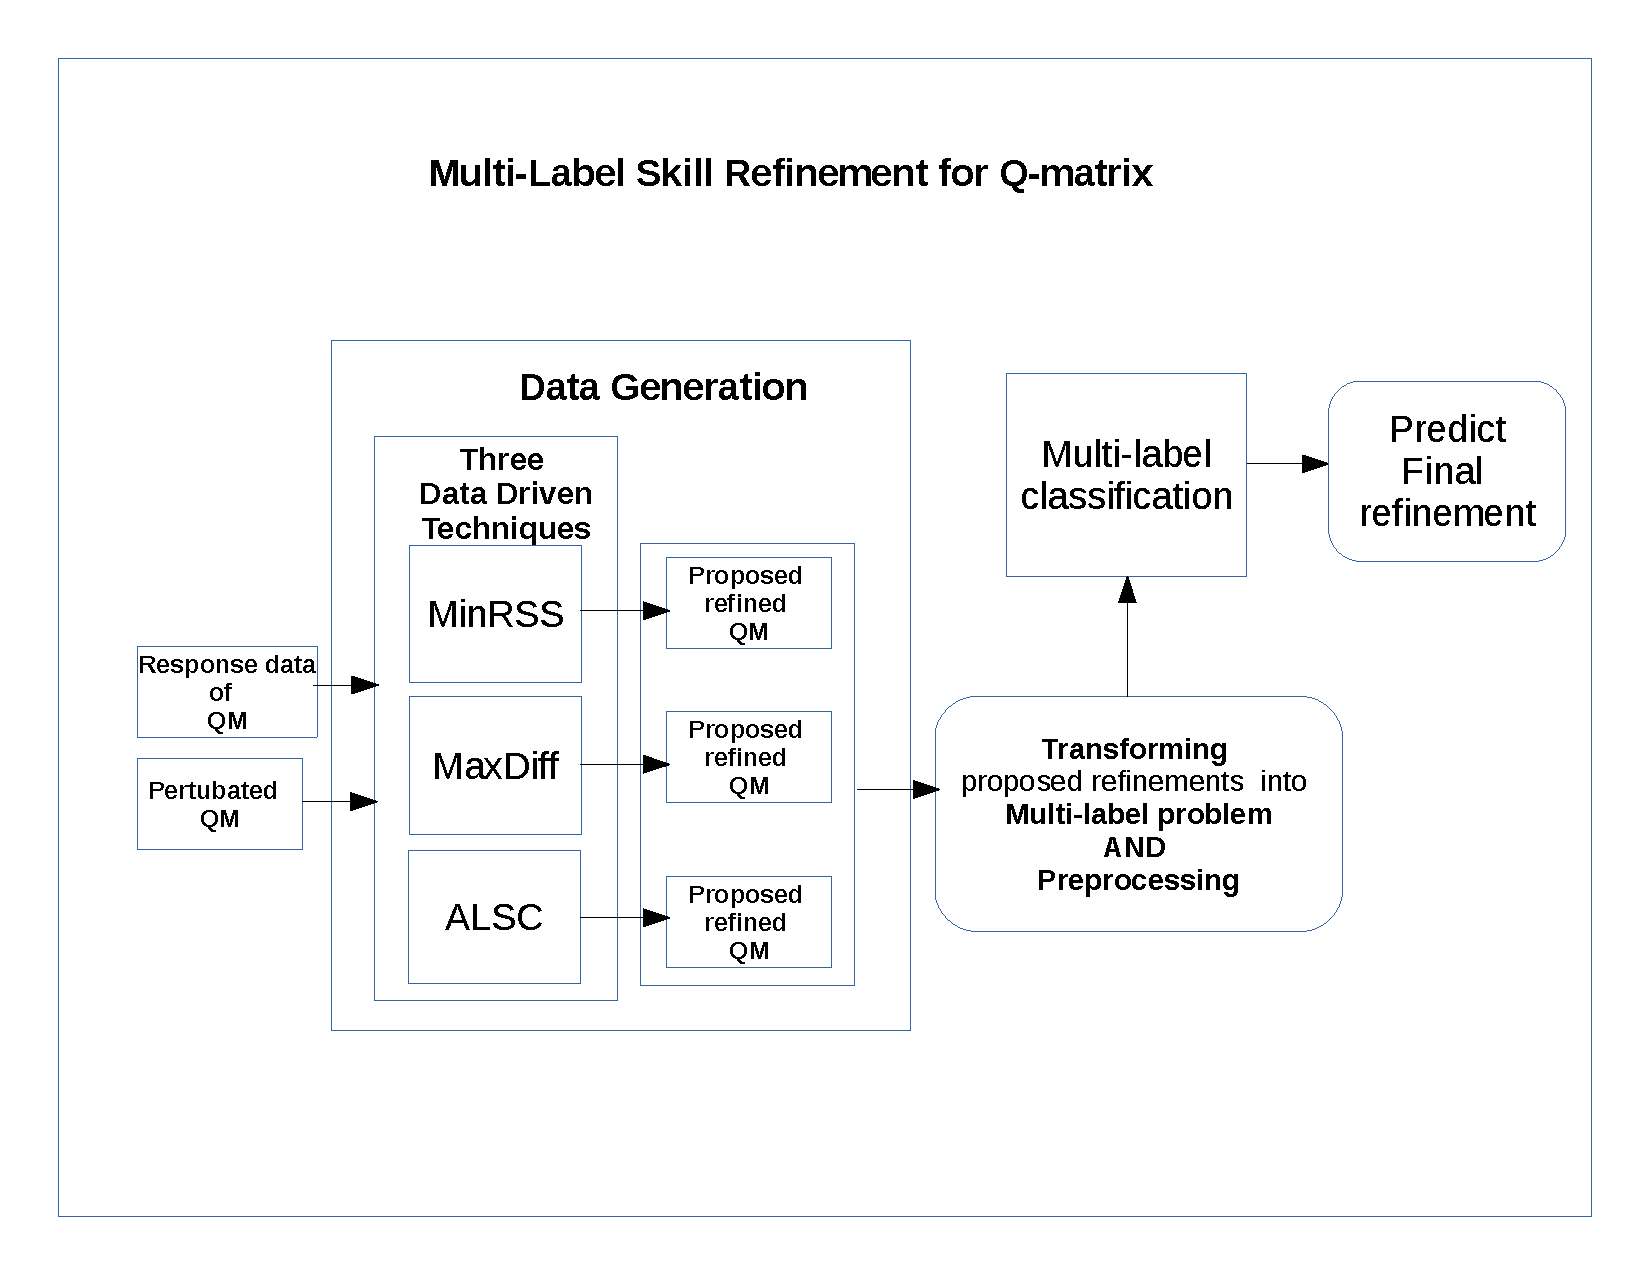
\includegraphics[width=100 mm ,scale=0.5]{graph/RP.pdf}
  \caption{Refinement Procedure of each Q-Matrix~$QM_i$ }
\end{figure} 

\subsection{Ensemble learning}

Ensemble methods use multiple learning algorithms to obtain better predictive performance. Desmarais et al. proposed a way to combine some techniques mentioned above in the framework of a decision tree \cite{desmarais2015combining}. For each record of the training set, the feature variables are composed of an entry of original Q-matrix and the proposed refined entry by different techniques. The target variable is the correspondent real Q-matrix entry. After training on this data set, the learned function is applied to real misspecified Q-matrix together with its refined Q-matrix offered by different techniques as the test set. However, this experiments explored only a single cell perturbation for training model and where test with both synthetic and real data (where real data was pertubated ranging from 1 to 10 cells).
%%%%%%%%%%%%%%%%%%%%%%%%%%%%%%%%%%%%%%%%%%%%%%%%%%%%%%%%%%%%%%%%%%%%%%%%%%%%%

\subsection{Data transformation and preprocessing}

Table~\ref{ref:data} contains an excerpt of data used to train the multi-label skills refinement algorithms.  Each line is a record for a single item to skills mapping.
The rightmost column contain the true labels. 
\begin{table}
\centering
	\begin{tabular}{c|ccccccccc|ccc}	
\toprule
\multirow{3}{*}{Items} & \multicolumn{9}{c}{Predicted Outputs skills $s_n$}\\
\cmidrule{2-9}
& \multicolumn{3}{c}{ MinRSS } & \multicolumn{3}{c}{MaxDiff}&\multicolumn{3}{c|}{ALSC}& \multicolumn{3}{c}{Real Values} \\ \\
\cmidrule{2-9}
& $s_1$ & $s_2$ & $s_3$ & $s_1$ & $s_2$ & $s_3$ & $s_1$ & $s_2$ & $s_3$  & \textbf{$s_1$} & \textbf{$s_2$} & \textbf{$s_3$}\\ \hline

	1 & 1 & 1 & 0 & 1 & 1 & 0 & 1 & 1 & 0  & 1 & 1 & 0 \\
	2 & 0 & 1 & 0 & 0 & 1 & 1 & 0 & 1 & 1 & 0 & 1 & 1 \\
	3 & 1 & 1 & 1 & 1 & 0 & 1 &1 & 1 & 1 & 1 & 0 & 1\\
	4 & 1 & 0 & 0 & 1 & 0 & 0 & 1 & 1 & 1 & 1 & 0 & 0 \\
	5 & 1 & 0 & 1 & 1 & 0 & 1 & 1 & 0 & 1  & 1 & 0 & 1\\
	... &... &... &... &... &... &... &... &... &... &...\\
	 \hline\hline
       
	\end{tabular}

\caption{Example of the data used for multi-label classification} \label{ref:data} 
\end{table}




\begin{figure}
  \centering
    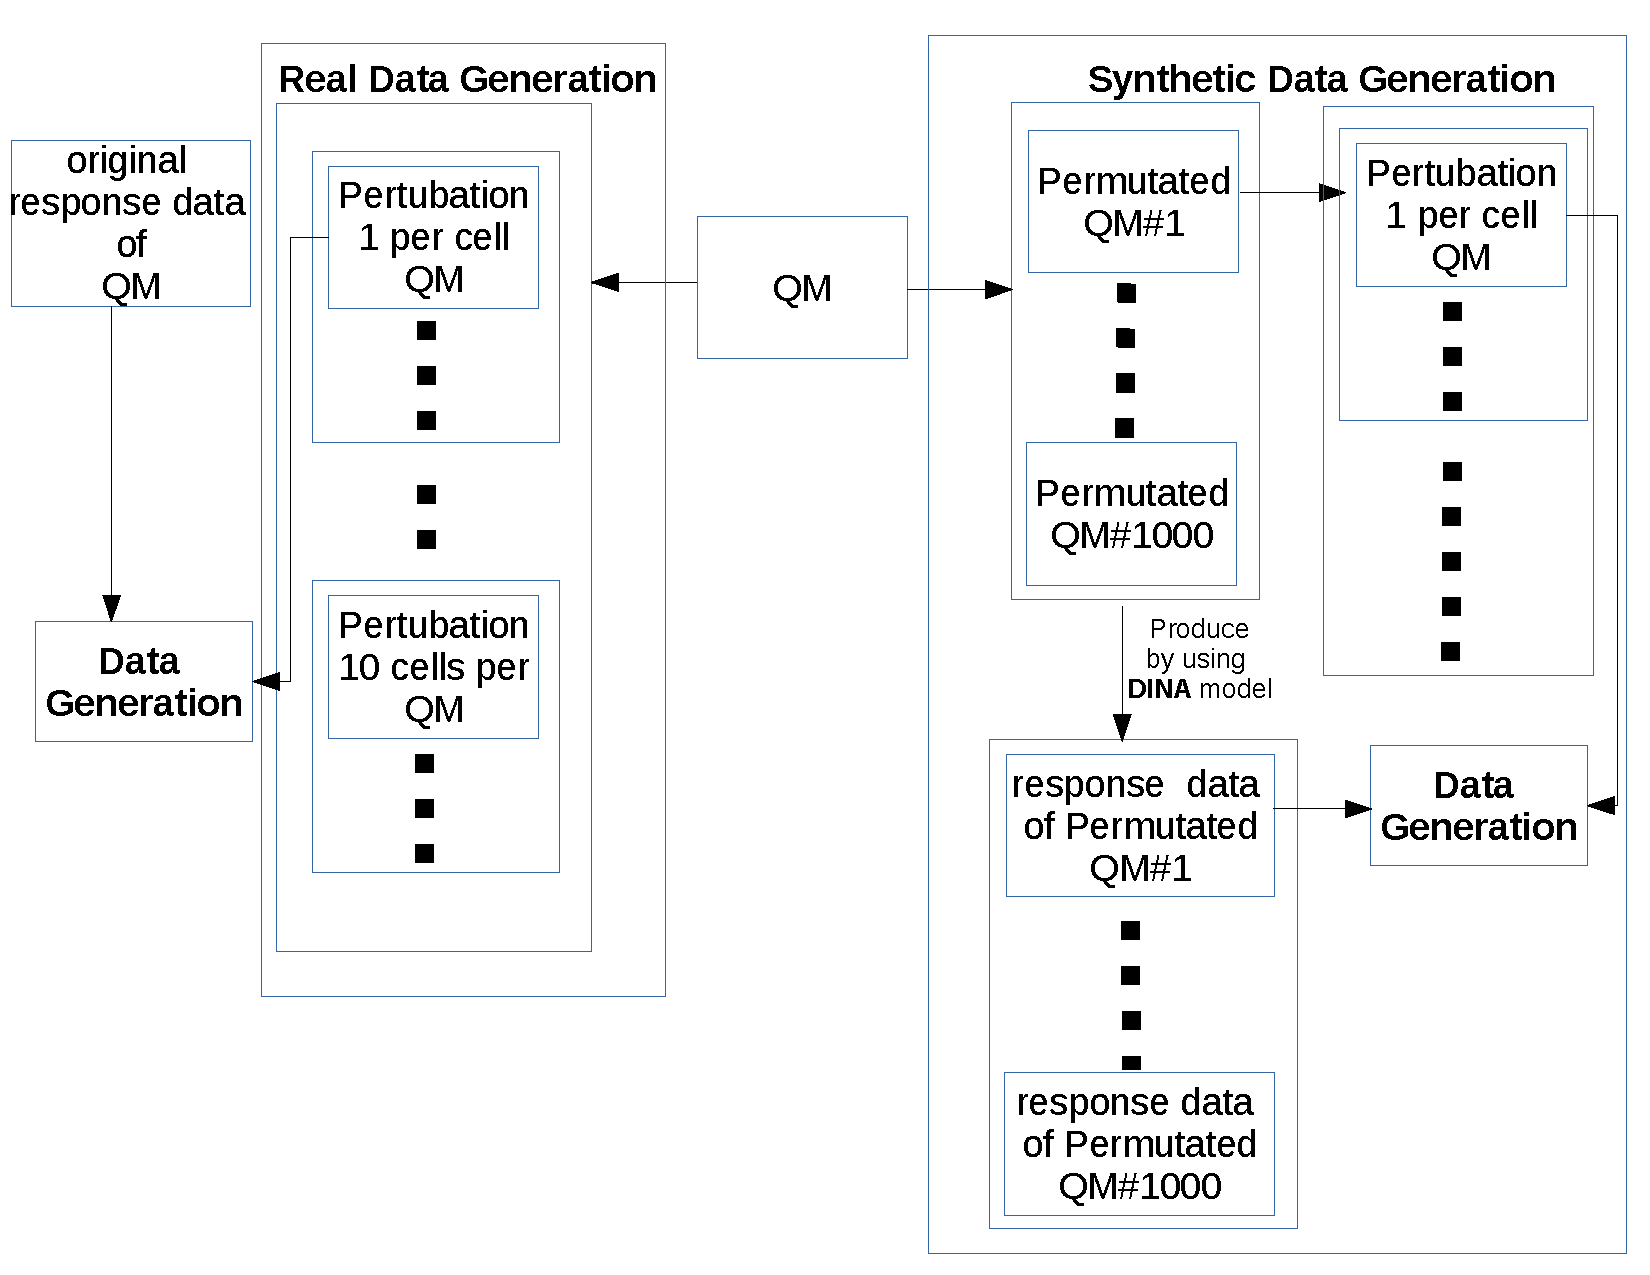
\includegraphics[width=100mm ,scale=0.5]{graph/DG.pdf}
  \caption{Data Generation Procedure of each Q-Matrix~$QM_i$}  \label{fig:DG}
\end{figure}

 we look for the most likely q-vector classes for training model by counting the frequencies of q-vectors proposed from three data driven techniques in real data. We choose q-vectors with frequencies larger than certain percentage(for eg. we used 5\% in this experiment). Only those most likely q-vectors are considered as classes in synthetic data for training model of multi-label classifiers .This is the most important step of this experiment.  

\subsection{muti-label skills refinement algorithms}

The generality of multi-label problems makes it significantly more complex to solve than traditional single-label (two-class or multi-class) problems. Only a few studies on multi-label learning are reported in the literature, which mainly concern the problems of text categorization, bioinformatics and scene classification. 

Multi-label classification aims to predict a whole vector of labels at once, namely the item skills set in our case. We have a vector of skills for each item in our Q-matrices. So we can transform the proposed outputs of Q-matrices driven from the three refinement techniques into multi-label classification problem and then we make final prediction by using those features. In this study, we use two multi-label classification methods: binary relevance method (Classifier chain method)~\cite{read2011classifier} by using Naive Bayes classifier, and RAndom k-labELsets(Ensemble method) \cite{Tsoumakas2011random} by using the J48 decision tree algorithm.

\subsubsection{Binary Relevance method with Naive Bayes}
The strategy of problem transformation is to use the one-against-all strategy by converting the multi-label problem into several binary classification problems. This approach is known as the binary relevance method (BR)~\cite{read2011classifier}. A method closely related to the BR method is the Classifier Chain method (CC) proposed by Read et al. \cite{read2011classifier}. This method involves~$Q$ binary classifiers linked along a chain. BR transforms any multi-label problem into one binary problem for each label. 

%% \add{\note{moved this paragraph here but needs to be double checked.}\label{notea}}
Let us introduce some notation. Given an instance~$X$ and its associated label set~$l_i \subset |L|$, where its~$l_i$ component of  $ |L|$ takes the value of 1 if~$l_i \in |L|$ and 0 otherwise. In addition, let~$N(x)$ denote the set of~$x$ identified in the training set.

Hence this method trains~$|L|$ binary classifiers~$C_1,...,C_{|L|}$. Each classifier~$C_j$ is responsible for predicting the~$0/1$ association for each corresponding label~$l_j \in L$.\\

BR with Naive Bayes (NB) method makes NB classifiers linked in a chain, such that the classifier for~$l_{i}$ in the chain considers the classes predicted~$l_1,l_2,...,l_{i-1}$ from the previous classifiers as additional attributes. Thus, the feature vector for each binary classifier is extended with the class values (labels) of all previous classifiers in the chain. Each classifier in the chain is trained to learn the association of label~$L_i$
given the features augmented with all previous class labels in the chain, $ C_1;C_1;C_2;...;C_{|L|}$. At classification time, the process starts at~$C_1$, and propagates the predicted classes along   the   chain   such   that   for~$C_i$ it   computes: 
\begin{equation}
P(l_i)= \arg \max_{l_i} P(l_i|X,l_1,l_2,...,l_{i-1}) 
\end{equation}

\subsubsection{RAndom k-labELsets with J48}
The ensemble methods for multi-label learning are developed on top of the common problem transformation or algorithm adaptation methods. The most well known problem transformation ensembles are the RAndom k-labELsets (RAkEL) system by Tsoumakas et al.~\cite{Tsoumakas2011random}. RAkEL constructs each base classifier by considering a small random subset of labels .It decompose all labels $L$ into $m$ random subsets of labels
with size $k$ and trains a label power-set classifier
using each set of labels. By using a simple voting process,it  determines the
final set of labels for a given example. In this way, the proposed algorithm aims to take into account label correlations using single-label classifiers that are applied on subtasks with a manageable number of labels and adequate number of examples per label. \\

In this experiment we use the single-label J48 classifier, an optimized  implementation of the  C4.5 or improved version of the  C4.5. J48 constructs a Decision tree as an output.  

\section{Empirical Study}

\subsection{Data}
For the sake of comparison, we use the same datasets as the ones used in Desmarais et al.\ (2015)~\cite{tatsuoka1983rule,desmarais2015combining}. It is a well known data set in
fraction algebra from Tatsuoka's work (Tatsuoka, 1984)\cite{tatsuoka1983rule}. It consists 3 expert-driven Q-matrices and one SVD driven Q-matrix with a same data set.These allow us to analyze possibility of different models (Q-matrices) over the same data source.Table~\ref{tab:qm} provides the basic information and source of each dataset.   






\begin{table}[h] 
\begin{center}
  \caption{Q-matrix for validation \& explanation of category}\label{tab:qm}
  \begin{tabular}{|ccccp{4cm}<{\raggedright}|}
  \hline
  \toprule
\multirow{2}{*}{Q-Matrices} & \multicolumn{3}{c}{Number of} & \multirow{2}{*|}{Description} \\
  \cline{2-4}
  & Skills &  Items & \multicolumn{1}{c}{Cases} & \\
  \midrule
QM1 & 3 & 11 & 536 & {Expert driven from \cite{henson2009defining} } \\
	\hline
QM2 & 5 & 11 & 536 & {Expert driven from \cite{de2008empirically} } \\  
 	\hline
QM3 & 3 & 11 & 536 & {Expert driven from \cite{CDM}} \\  
  	\hline 
QM4 & 3 & 11 & 536 & {Data driven, SVD based} \\  
  	\hline
  	\end{tabular}  
\end{center}	
\end{table}





\subsection{Error metric}\label{sec:eval-meas-princ}

%% \add{\note{is this notation consistent with the above (note~\ref{notea})?}}
The evaluation of methods for multi-label data requires different metrics than those used in the case of single label data. For the definitions of these metrics, we will consider an evaluation data set of multi-label examples~$(x_i ,Y_i ), i = 1...m, $ where~$ Y_i \subseteq L~$ is the set of true labels and~$ Z_i~$ is the set of predicted labels. This section presents some metrics: Hamming loss, Subset Accuracy and Example based F-measure \cite{Tsoumakas2010MLD} that will be used in this experiment to
assess the performance of the different algorithms. 
%\item Ranking based measurement: are measured based on the ranking scores they received and how far with %respect to the ground truth of multi-label data. It concludes with a subsection on measures that take into %account label hierarchy of the existing label sets. The highest rank is received by the most relevant %label, while the least relevant one, receives the lowest rank.


%% MD: to validate by Sein Minn
%% \subsubsection{Example based metric}
%% %% \add{\note{Single section here}}
%% Example based metrics are calculated over all examples of the evaluation data set, that based on the average differences of the actual and the predicted sets of labels.

\subsubsection{Hamming Loss} a measure of how many times an instance label set is misclassified, i.e. a label not belonging to the instance is predicted or a label belonging to the instance is not predicted. The performance is perfect when~$Hamming Loss=0$; the smaller the value of~$Hamming Loss$, the better the performance:
\begin{equation} 
 Hamming Loss= \frac{1}{m}\sum_{i=1}^{m}  \frac{|Z_i\Delta Y_i|}{M}
\end{equation}
where~$\Delta$ stands for the symmetric difference between two label sets. which is the theoretic equivalent of the exclusive disjunction (XOR operation) in Boolean logic for sets.
\subsubsection{Accuracy}
 Accuracy is to calculate the accuracy of vector of labels is truly classified. $ Accuracy$ is defined as follows:
\begin{equation} 
 Accuracy= \frac{1}{m}\sum_{i=1}^{m}  I(Z_i = Y_i)
\end{equation}
\subsubsection{F-score} F-score is calculated based on the average differences of the actual and the predicted sets of labels over all examples of the evaluation data set. The performance is perfect when~$F-score = 1$; the bigger the value ,the better the performance:
\begin{equation} 
 Example based F-score= \frac{1}{m}\sum_{i=1}^{m} \frac{2|Y_i \cap Z_i|}{|Z_i|+|Y_i|}
\end{equation}
%%%%%%%%%%%%%%%%%%%%%%%%%%%%%%%%%%%%%%%%%%%%%%%%%%%%%%%%%%%%%%%%%%%%%%%%%%%%%
\section{Result}

The experimental results are reported in Tables [\ref{ref:Syn_HL},\ref{ref:Syn_SA},\ref{ref:Syn_FM}] for synthetic data, and in  Figures [\ref{fig:HLforReal},\ref{fig:SAforReal},\ref{fig:FMforReal}] for real data. Four variations of the two multi-label approaches are reported for both real and synthetic data (BR and RAkEL).
\subsection{Result for synthetic data}



\begin {table}[h]
\scriptsize
\centering
\begin{tabular}{c|c|c|c|c|c}	
	\hline\hline	
QM & MinRSS & MaxDiff & ALSC & RAkEL & BR   \\ \hline
qm1 & 0.01 & 0.02 & 0.01 & 0.00 & 0.00 \\
qm2 & 0.02 & 0.04 & 0.06 & 0.01 & 0.01  \\
qm3 & 0.00 & 0.02 & 0.01 & 0.00 & 0.00   \\
qm4 & 0.01 & 0.02 & 0.01 & 0.00 & 0.01  \\  \hline\hline
\end{tabular}
\caption {Hamming Loss result of Synthetic data (single perturbation)} \label{ref:Syn_HL} 
\end{table}




\begin {table}[h]
\scriptsize
\centering
\begin{tabular}{c|c|c|c|c|c}	
	\hline\hline	
QM  & MinRSS  & MaxDiff  & ALSC  & RAkEL & BR    \\  \hline
qm1  & 0.98 & 0.95 & 0.97 & 0.99 & 0.99  \\
qm2  & 0.90 & 0.83 & 0.72 & 0.97 & 0.94  \\
qm3  & 0.99 & 0.96 & 0.99 & 1.00 & 1.00  \\
qm4  & 0.98 &  0.94 & 0.98 & 0.99 & 0.98  \\
\hline\hline
\end{tabular}
\caption {SubSet Accuracy result of Synthetic data (single perturbation)} \label{ref:Syn_SA} 
\end{table}



\begin {table}[h]
\scriptsize
\centering
\begin{tabular}{c|c|c|c|c|c}	
	\hline\hline	
 QM  &  MinRSS & MaxDiff  &  ALSC  &  RAkEL &  BR  \\ 
 qm1  & 0.99 & 0.98 & 0.99 & 1.00 & 1.00  \\  
 qm2  & 0.98 & 0.98 & 0.96 & 1.00 & 0.99  \\
 qm3  & 1.00 & 0.98 & 0.99 & 1.00 & 1.00  \\
 qm4  & 0.99 & 0.98 & 0.99 & 1.00 & 0.99  \\
\hline\hline
\end{tabular}
\caption {Macro averaged F-measure result of Synthetic data (single perturbation)} \label{ref:Syn_FM} 
\end{table}

All experiments were done with 10 fold cross validation.

 
 For synthetic data, a single cell is perturbed. We can see from Tables [4,5,6]
that most of multi-label skill refinement methods can recover 99\% for all
Q-matrices and even the performance reaches 100\% in terms of accuracy
and F-measure. The standard deviations of all values are less than 0.00, so we do not mention in here. Clearly, all methods using multi-label refinement algorithms perform much better than any single method and the results are also substantially better than those of the single-cell decision tree method reported in~\cite{desmarais2015combining}. It is more significant when q-vector contains more skills.(for eg., QM2 has 5 skills while others have only 3 skills. In this case, the porposed method singnificantly outperform than other methods). 




\subsection{Result for real data}
For real data, multiple perturbations are introduced and the results are shown as figures to better visualize the trends as a function of the number of perturbations.   A logit scale is used which can be considered a good estimate of the relative remaining error on a scale of~$[0,1]$ (for eg., it displays a relative error reduction in accuracy from~0.90 to~0.95 as similar to the reduction from~0.99 to~0.995). The black lines show the results of the three individual refinement algorithms, and the coloured lines show the multi-label algorithms results.  

As expected, the performance of all methods decline with the number of perturbations. The prposed methods show more significant performance than three data driven method along with the number of petubation. RAkEL shows the best performances for expert driven Q-matrices in general, but not that signifcant for SVD driven Q-matrix. However, the results for QM3 and QM4 shows that the MaxDiff method has better performance than proposed methods up to 3 or 4 pertubations, but proposed methods can recover the QMs more effectively and accurately when it contains more errors in those QMs.



\begin{figure}
  \centering
    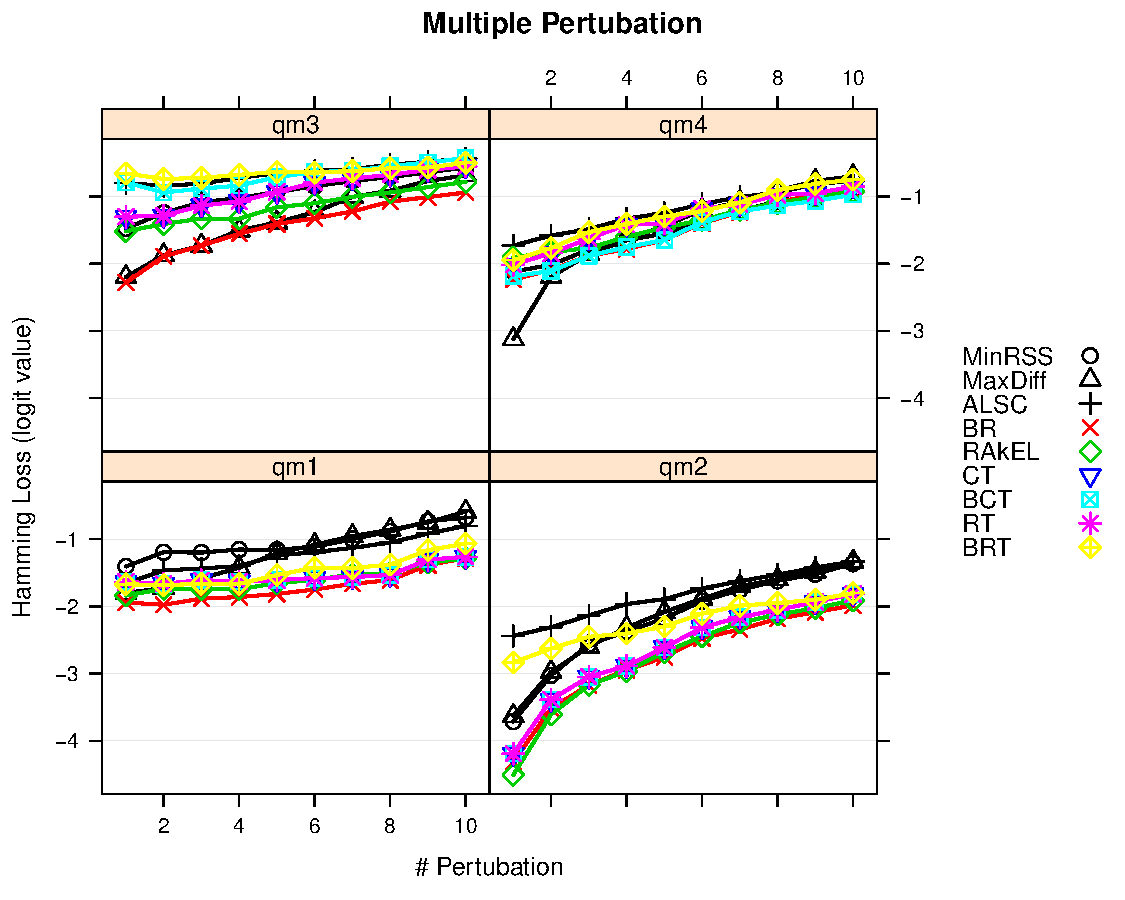
\includegraphics[width=100 mm ,scale=0.25]{graph/HL.pdf}
  \caption{Real data: Logit value of Hamming loss as a function of the number of perturbations}\label{fig:HLforReal}
\end{figure}

\begin{figure}
  \centering
    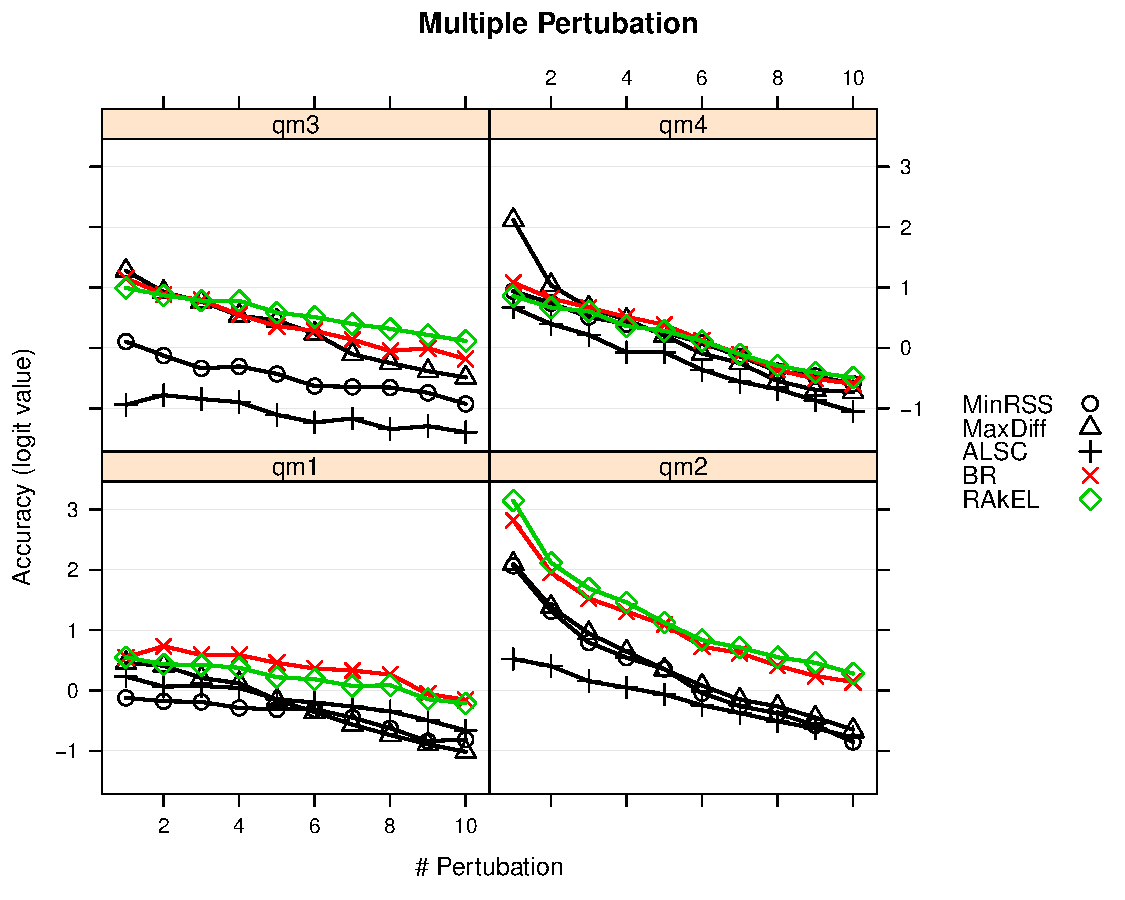
\includegraphics[width=100 mm ,scale=0.25]{graph/SA.pdf}
  \caption{Real data: Logit value of Subset Accuracy as a function of the number of perturbations}\label{fig:SAforReal}
\end{figure}

\begin{figure}
  \centering
    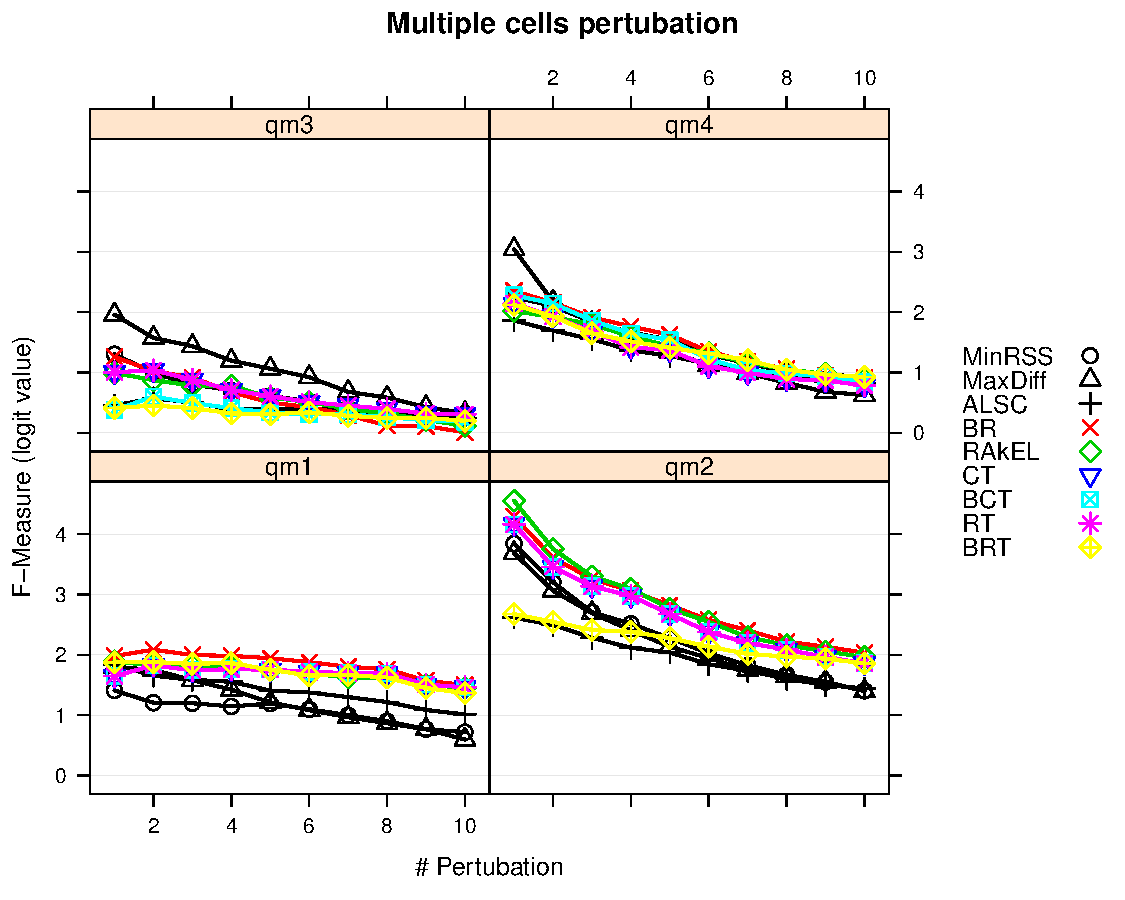
\includegraphics[width=100 mm ,scale=0.25]{graph/FM.pdf}
    \caption{Real data: Logit value of Example-based F-measure as a function of the number of perturbations}\label{fig:FMforReal}
\end{figure}



%%%%%%%%%%%%%%%%%%%%%%%%%%%%%%%%%%%%%%%%%%%%%%%%%%%%%%%%%%%%%%%%%%%%%%%%%%%%%
\section{Conclusion}
We proposed multi-skill refinement method to improve the performance of traditional  algorithms on Q-matrix validation problem. In this proposal, we apply ensemble technique that based on multi-lable classification to choose the correct skills in q-vectors by using the proposed q-vectors from three data driven techniques as features. In where, classification model was trained by vast amount of permutated Q-matrices produced synthetically. This model provides the decision about whether what skills in q-vectors are correctly specified and refined simulataneously (if necessary)  by accessing the results proposed by three data driven methods as features for real data. It can be seen as to improving the performance of Q-matrix refinement algorithms by using a supervised model trained by huge amout of all possible q-vectors form pemutated Q-matrices. The results reveal the proposed method provide better performance than existing algorithms and it is more significat when Q-matrices contain more errors. Otherwise, the proposed methods are more likely to outperform when dealing Q-matrices with larger number of skills.  


%%%%%%%%%%%%%%%%%%%%%%%%%%%%%%%%%%%%%%%%%%%%%%%%%%%%%%%%%%%%%%%%%%%%%%%%%%%%%
\section{Future Work}

In this porposal, we are only dealing with Q-matrix that show what skill are required for what kind of tasks by using binary values. In future, we are going to deal with Q-matrices revealing skills requirement with multiple level of proficiency  for each task.Besides,we are only dealing with the static data that is the snapshot data extracted from student examination. we are going to deal with dynamic data that is extracted form tutoring system. In where, students were asked the specific questions serveral times and their performace would be improved when the students learn skills required according to time period. We are going to dealing with such data that change over time. We are passinate about learning how a student learn their skills required for their tasks according to time.  

\bibliographystyle{apacite}
\bibliography{Proposal}
\end{document}
